\subsection{Đề 03}
\Opensolutionfile{ans}[ans/ans-CTST_0-OTGK1_De03-LC]
\caulc
\begin{ex}%[Nguyễn Tuấn, sáng tác đề HK1 Khối 10]%[0D1N1-1]
	Trong các câu dưới đây, câu nào là một mệnh đề?
	\choice
	{$\sqrt{2}$ có phải là số vô tỉ không?}
	{\True Tây Ban Nha là đội tuyển vô địch Euro 2024}
	{Bạn là học sinh trường nào?}
	{Thời tiết hôm nay thật đẹp!}
	\loigiai{
		\lq\lq Tây Ban Nha là đội tuyển vô địch Euro 2024 \rq\rq \,là một câu khẳng định có tính đúng sai nên là một mệnh đề.
	}
\end{ex}
\begin{ex}%[Nguyễn Tuấn, sáng tác đề HK1 Khối 10]%[0D1N2-1]
	Cho tập hợp $A=[1;5]$, phát biểu nào sau đây đúng?
	\choice
	{$A=\{x\in\mathbb{N}\mid 1\le x\le 5\}$}
	{\True$A=\{x\in \mathbb{R}\mid 1\le x\le 5\}$}
	{$A=\{1;2;3;4;5\}$}
	{$A=\{1;5\}$}
	\loigiai{
		\begin{itemize}
			\item $A=[1;5]$ có các phần tử là số thực $\mathbb{R}$ nên loại đáp án $A=\{1;2;3;4;5\}$ và $A=\{x \in \mathbb{N}\mid 1 \le x \le 5\}$.
			\item $A=\{1;5\}$ sai.
			\item Đáp án $A=\{x \in \mathbb{R}\mid 1 \le x \le 5\}$ đúng.
		\end{itemize}
	}
\end{ex}
\begin{ex}%[Nguyễn Tuấn, sáng tác đề HK1 Khối 10]%[0D1N3-2]
	Cho hai tập hợp $A=\{1;2;3;4;5\}$ và $B=\{2;4;6;7;8\}$. Tìm $A\setminus B$.
	\choice{$A\setminus B=\{1;2;3;4;5;6;7;8\}$}
	{$A\setminus B=\{2;4\}$}
	{$A\setminus B=\{6;7;8\}$}
	{\True$A\setminus B=\{1;3;5\}$}
	\loigiai{
		Ta có $A\setminus B=\{1;3;5\}$.
	}
\end{ex}
\begin{ex}%[Nguyễn Tuấn, sáng tác đề HK1 Khối 10]%[0D1H3-3]
	Cho hai tập hợp $A=(-\infty;3]$ và $B=(1;10]$. Khi đó, tập $A\cup B$ là
	\choice
	{$(1;3]$}
	{$(3;10]$}
	{\True $(-\infty;10]$}
	{$(-\infty;1)$}
	\loigiai{\immini{Ta có $A\cup B=(-\infty;10]$.}
		{	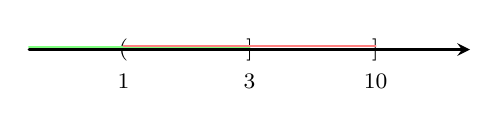
\begin{tikzpicture}[font=\footnotesize, line join=round, line cap=round, >=stealth,scale=0.8]
				\draw [line width=1pt] [->] (-0.5,0)--(6.5,0);
				\large
				\draw (1,0) node {(};
				\draw (3,0) node {]};
				\draw (5,0) node {]};
				\normalsize
				\draw (1,-0.5) node {$1$};
				\draw (5,-0.5) node {$10$};
				\draw (3,-0.5) node {$3$};
				\draw[color=green!50,thick] (-0.5,0.035)--(3,0.035);
				\draw[color=red!50,thick] (1,0.06)--(5,0.06);
		\end{tikzpicture}}
} \end{ex}
\begin{ex}%[Nguyễn Tuấn, sáng tác đề HK1 Khối 10]%[0D2N1-2]
	Miền nghiệm của bất phương trình $x+2y-4<0$ là nửa mặt phẳng không chứa điểm nào trong các điểm sau?
	\choice
	{$(0;0)$}
	{$(1;1)$}
	{\True $(4;3)$}
	{$(1;-1)$}
	\loigiai{
		Xét điểm $(4;3)$. Ta có $4+2\cdot 3-4=6<0$ (sai).\\
	Vậy miền nghiệm của bất phương trình $x+2y-4<0$ là nửa mặt phẳng không chứa điểm $(4;3)$.
	}
\end{ex}
\begin{ex}%[Nguyễn Tuấn, sáng tác đề HK1 Khối 10]%[0D2N2-1]
	Hệ bất phương trình nào sau đây là hệ bất phương trình bậc nhất hai ẩn?
	\choice
	{$\heva{&x+y-4xy>3\\&3x-4y\le5}$}
	{\True $\heva{&3x+y\le1\\&x-2y>4}$}
	{$\heva{&5x-4y\ge0\\&(x-3)y\le1}$}
	{$\heva{&1-2xy>3\\&3x-y\le7}$}
	\loigiai{Ta thấy $\heva{&3x+y\le1\\&x-2y>4}$ là một hệ bất phương trình bậc nhất hai ẩn.}
\end{ex}
\begin{ex}%[Nguyễn Tuấn, sáng tác đề HK1 Khối 10]%[0D3N1-2]
	Tập xác định của hàm số $y=\sqrt{x-7}$ là
	\choice
	{$(-\infty;7]$}
	{$(-\infty;7)$}
	{$(7;+\infty)$}
	{\True $[7;+\infty)$}
	\loigiai{
		Hàm số xác định khi $x-7\ge 0\Leftrightarrow x\ge 7$.\\
		Vậy tập xác định của hàm số là $\mathscr{D}=[7;+\infty)$.}
\end{ex}
\begin{ex}%[Nguyễn Tuấn, sáng tác đề HK1 Khối 10]%[0D3H1-3]
	Cho hàm số $f(x)= x^2+kx-5$, với $k$ là hằng số. Nếu $f(-2)=3$ thì giá trị của $f(2)$ là bao nhiêu?
	\choice
	{\True $-5$}
	{$-3$}
	{$3$}
	{$5$}
	\loigiai{
		Ta có
		$f(-2)=3\Leftrightarrow (-2)^2+k\cdot (-2)-5 = 3\Leftrightarrow k=-2$. \\
		Khi đó $f(x)=x^2-2x-5$.\\
		Vậy $f(2)=-5$.
	}
\end{ex}
\begin{ex}%[Nguyễn Tuấn, sáng tác đề HK1 Khối 10]%[0H4N1-1]
	Cho $\alpha $ là góc tù. Khẳng định nào sau đây là đúng?
	\choice
	{$\sin \alpha <0$}
	{$\cos \alpha >0$}
	{\True $\tan \alpha <0$}
	{$\cot \alpha >0$}
	\loigiai{
		Góc tù có điểm biểu diễn thuộc góc phần tư thứ II, có giá trị $\sin \alpha >0$, còn $\cos \alpha$, $\tan \alpha$ và $\cot \alpha$ đều nhỏ hơn $0$.
	}
\end{ex}
\begin{ex}%[Nguyễn Tuấn, sáng tác đề HK1 Khối 10]%[0H4N2-1]
	Cho tam giác $ABC$, mệnh đề nào sau đây đúng?
	\choice
	{$a^2= b^2+c^2+2bc\cos A$}
	{\True $a^2= b^2+c^2 - 2bc\cos A$}
	{$a^2= b^2+c^2-2bc\cos C$}
	{$a^2= b^2+c^2- 2bc\cos B$}
	\loigiai
	{
		Theo định lí cosin trong tam giác $ABC$, ta có $a^2= b^2+c^2-2bc \cos A$.
	}
\end{ex}
\begin{ex}%[Nguyễn Tuấn, sáng tác đề HK1 Khối 10]%[0H4N3-1]
	Cho tam giác $ABC$ có diện tích bằng $24$ và chu vi bằng $24$. Bán kính $r$ của đường tròn nội tiếp tam giác $ABC$ là?
	\choice
	{$r=\dfrac{1}{2}$}
	{$r=1$}
	{$r=3$}
	{\True $r=2$}
	\loigiai{
		Ta có $p=\dfrac{24}{2}=12$.\\
		Ta có $S=p\cdot r\Rightarrow r=\dfrac{S}{p}=2$.}
\end{ex}
\begin{ex}%[Nguyễn Tuấn, sáng tác đề HK1 Khối 10]%[0H4H3-2]
	\immini[thm]
{
	Trên sườn đồi có một cái cây thẳng đứng (tham khảo hình vẽ) đổ bóng dài $AB=39{,}5$ mét xuống đồi. Biết góc nghiêng của sườn đồi là $\alpha =26^\circ$ so với phương ngang và góc nâng của mặt trời là $\beta =50^\circ$.
	Chiều cao $BC$ của cây (làm tròn đến hàng đơn vị) là
	\choice
	{$21$ m}
	{$27$ m}
	{\True $25$ m}
	{$23$ m}
}{
	\begin{tikzpicture}[scale=0.8,font=\footnotesize, line join=round, line cap=round, >=stealth]
		\path 
		(0,0) coordinate (O)
		(-3,0) coordinate (A)
		(0,4) coordinate (C)
		($(A)!1!26:(O)$) coordinate (b)
		(intersection of A--b and O--C) coordinate (B);
		;
		
		\begin{scope}[shift={(B)}]
			\fill[blue!50!yellow] (-.1,0) rectangle (.1,1);
			\foreach \x/\y/\z in {1/.6/1.2,.9/.8/1.4,.8/1/1.6,.7/1.2/1.8,.6/1.4/2,.5/1.6/2.2,.4/1.8/2.5}
			{
				\fill[green!50!black] 
				(-\x,\y)--(\x,\y)--(0,\z)--cycle;
			}
			
		\end{scope}
		\draw[dashed] (A)--(O)--(C)--cycle;
		\draw[line width=1.2pt,shorten <=-1cm,shorten >=-1cm] (A)--(b);
		\draw[dashed,shorten >=-1cm] (A)--(C);
		\pic[draw,"$\alpha$", angle eccentricity=1.3,angle radius=0.5cm]{angle=O--A--B};
		\pic[draw,below,"$\beta$", angle eccentricity=1.3,angle radius=1cm]{angle=O--A--C};
		\draw pic[draw, angle radius=2mm]{right angle=A--O--C};
		\foreach \x/\g in {A/-90,C/0,B/-50,O/0} \fill[black] (\x) circle (1pt)+(\g:.3) node {$\x$};
		\begin{scope}[shift={($(C)+(1,1.3)$)}]
			\fill[orange!30!yellow] (0,0) circle (.5cm);
			\foreach \i in {0,30,60,...,360}{
				\begin{scope}[rotate=\i]
					\draw[orange!30!yellow,line width=1pt] (.7,0)--(1,0);
			\end{scope}}
		\end{scope}
		
	\end{tikzpicture}
}
\loigiai{
	Ta có $\widehat{BAC}=\widehat{OAC}-\widehat{OAB}=24^\circ$ và $\widehat{BCA}=90^\circ-50^\circ=40^\circ$.\\
	Áp dụng định lý sin trong $\triangle ABC$, ta có
	\allowdisplaybreaks
	\begin{eqnarray*}
		&&\dfrac{BC}{\sin\widehat{BAC}}=\dfrac{AB}{\sin\widehat{ACB}}\\
		&\Rightarrow& BC=\dfrac{AB\cdot\sin\widehat{BAC}}{\sin\widehat{ACB}}\\
		&\Rightarrow& BC=\dfrac{39{,}5\cdot\sin 24^\circ}{\sin 40^\circ}\approx 25 ~(\text{m}).
	\end{eqnarray*}
}
\end{ex}
\Closesolutionfile{ans}
\indapan{6}{ans/ans-CTST_0-OTGK1_De03-LC}
%-------------------------------------------
\Opensolutionfile{ans}[ans/ans-CTST_0-OTGK1_De03-DS]
\cauds
\begin{ex}%[Nguyễn Tuấn, sáng tác đề HK1 Khối 10]%[0D1H3-2]
	Cho tập hợp $A=\left\{n \in \mathbb{N}\big|2n+1\le 17\right\}$, $B=\left\{n\in \mathbb{N} \big| n^2 \le 25\right\}$.
	\choiceTF
	{\True $A=\{0;1;2;3;4;5;6;7;8\}$}
	{Tập $B$ có $5$ phần tử}
	{\True Tập hợp $A\cap B$ có $6$ phần tử}
	{$B\setminus A= \{6;7;8\}$}
	\loigiai{
		\begin{itemchoice}
			\itemch {\bf Đúng}. Ta có $2n+1 \le 17 \Leftrightarrow n\le 8$. Mà $n\in \mathbb{N}$ nên $A=\{0; 1; 2; 3; 4; 5; 6; 7; 8\}$.
			\itemch {\bf Sai}. Ta có $n^2 \le 25 \Leftrightarrow n\le 5$. Mà $n\in \mathbb{N}$ nên $B= \{0; 1; 2; 3; 4; 5\}$. Tập $B$ có $6$ phần tử.
			\itemch {\bf Đúng}. Ta có $A\cap B= \{0; 1; 2; 3; 4; 5\}$. Do đó $A\cap B$ có $6$ phần tử.
			\itemch {\bf Sai}. Ta có $B\setminus A= \varnothing$.
		\end{itemchoice}
	}
\end{ex}
%\begin{ex}%[Nguyễn Tuấn, sáng tác đề HK1 Khối 10]%[0D2V2-3]
%	Bác An dự định trồng hai loại cây ăn trái là mít và xoài trong nông trại rộng $100$ hecta. Biết mỗi hecta trồng mít cần $20$ công chăm sóc và thu lại lợi nhuận $150$ triêu đồng, mỗi hecta trồng xoài cần $40$ công chăm sóc và thu lại lợi nhuận $180$ triệu đồng. Biết rằng tổng số công cần dùng không được vượt quá $2\,800$ công. Gọi $x$, $y$ (hecta) lần lượt là diện tích đất dùng để trồng mít và xoài. Xét tính đúng sai các phát biểu sau
%	\choiceTF
%	{\True $x+y \le 100$}
%	{\True $x+2 y \le 140$}
%	{\True Tổng lợi nhuận thu được là $F=150 x+180 y$ (triệu đồng)}
%	{Lợi nhuận thu được lớn nhất là $16$ tỷ đồng}
%	\loigiai{
%		\begin{itemchoice} 
%			\itemch {\bf Đúng}. Ta có $x+y\le 100$.
%			\itemch {\bf Đúng}. Số công cần dùng là $20x+40y \le 2\,800$ hay $x+2y\le 140$.
%			\itemch {\bf Đúng}. Tổng số tiền thu được là $F=150x+180y$ (triệu đồng).
%			\itemch {\bf Sai}. Điều kiện $x \ge0$, $y \ge 0$.\\
%			Nên ta cần tìm $x$, $y$ thỏa mãn hệ bất phương trình $\heva{& x \ge 0 \\ & y \ge 0 \\ & x+y \le 100 \\ & x+2 y \le 140}$ sao cho $F=150 x+180 y$ lớn nhất.\\
%			Biểu diễn tập nghiệm của hệ bất phương trình trên ta được miền tứ giác $OABC$ (kể cả biên) với $A(0;70)$, $B(60;40)$, $C(100;0)$ và $O(0;0)$ như hình bên dưới
%			\begin{center}
%				\begin{tikzpicture}[line join=round, line cap=round,>=stealth,thick,scale=.6]
%					\tikzset{every node/.style={scale=0.9},
%						declare function={x1=-1.5;x2=12.5;y1=-1.5;y2=11.5;}
%					}
%					\tikzset{declare function={
%							a=-1;b=10;
%							f(\x)=a*(\x)+b;
%							a2=-1/2;b2=7;
%							g(\x)=a2*(\x)+b2;	
%							a3=-1/4;b3=6;
%							h(\x)=a3*(\x)+b3;	
%					}}
%					\begin{scope}
%						\clip (x1,y1)rectangle (x2-.3,y2-.3);
%						\draw[smooth,samples=100,domain=x1:x2]plot(\x,{f(\x)});
%						\fill[pattern=north west lines] plot[domain=x1:x2](\x,{f(\x)})--(x2,y2)--(x1,y2);
%						
%						\draw[smooth,samples=100,domain=x1:x2]plot(\x,{g(\x)});
%						\fill[pattern=north west lines] plot[domain=x1:x2](\x,{g(\x)})--(x2,y2)--(x1,y2);
%					
%						\filldraw[pattern=north west lines] (x1-.1,y1-.1)rectangle(x2,0);
%						\filldraw[pattern=north west lines] (x1-.1,y1-.1)rectangle(0,y2);
%					\end{scope}
%					\draw[->] (x1,0)--(x2,0)node[above]{$x$};
%					\draw[->](0,y1)--(0,y2)node[left]{$y$};
%					\filldraw[black] (0,0)circle(1.2pt)node[below left]{$O$};
%					\foreach \x/\goc in {1,2,3,4,5,6,7,8,9,10}{
%						\draw (\x,.15)--(\x,-.15)node[below]{$\x0$};	
%					}
%					\draw 
%					(0,7)circle(1pt)node[above right,scale=.8]{$A$} 
%					(6,4)circle(1pt)node[above right,scale=.8]{$B$}
%					(10,0)circle(1pt)node[above right,scale=.8]{$C$}
%					%		(7,0)circle(1pt)node[above right,scale=.8]{$D$}		
%					;
%					\foreach \y/\goc in {1,2,3,4,5,6,7,8,9,10}{
%						\draw (.15,\y)--(-.15,\y)node[left]{$\y0$};	
%					}
%				\end{tikzpicture}
%			\end{center}
%			Biểu thức $F=150x+180y$ đạt giá trị lớn nhất tại $(x;y)$ là tọa độ một trong các đỉnh của tứ giác $OABC$.\\
%			Ta có
%			$F(0;0)=0$, $F(0;70)=12\,600$, $F(100;0)=15\,000$, $F(60;40)=16\,200$.\\
%			Khi đó giá trị lớn nhất tại $B(60; 40)$ nghĩa là bác Long cần trồng $60$ hecta mít và $40$ hecta xoài thì thu được lợi nhuận lớn nhất là $16{,}2$ tỷ đồng.
%	\end{itemchoice}}
%\end{ex}
\begin{ex}%[Nguyễn Tuấn, sáng tác đề HK1 Khối 10]%[0D3H1-4]
	Cho $4$ hàm số
	\begin{enumEX}[1)]{2}
		\item $f(x)=\dfrac{2x+3}{x^2}$.
		\item $g(x)=\dfrac{x^2+2}{x}$.
		\item $h(x)=x^3+3x^2-1$.
		\item $k(x)=\dfrac{x+2}{x-1}$.
	\end{enumEX}
	\choiceTF
	{\True Chỉ có $1$ hàm số có tập xác định là $\mathbb{R}$}
	{\True Đồ thị hàm số $f(x)$ đi qua điểm $(1;5)$}
	{\True Hàm số $k(x)$ nghịch biến trên các khoảng xác định}
	{Có $2$ điểm có tọa độ nguyên thuộc đồ thị hàm số $g(x)$}
	\loigiai{
		\begin{itemchoice}
			\itemch {\bf Đúng}. Ta có 
			\begin{itemize}
				\item $y=\dfrac{2x+3}{x^2}$ có tập xác định là $\mathscr{D}=\mathbb{R}\setminus\{0\}$.
				\item $y=\dfrac{x^2+2}{x}$ có tập xác định là $\mathscr{D}=\mathbb{R}\setminus\{0\}$.
				\item $y=x^3+3x^2-1$ có tập xác định là $\mathscr{D}=\mathbb{R}$.
				\item $y=\dfrac{x+2}{x-1}$ có tập xác định là $\mathscr{D}=\mathbb{R}\setminus\{1\}$.
			\end{itemize}
			Vậy  hàm số $y=x^3+3x^2-1$ có tập xác định là $\mathscr{D}=\mathbb{R}$.
			\itemch {\bf Đúng}. Thay $x=1$ vào hàm số $f(x)$ ta có $f(1)=5$.\\ 
			Vậy đồ thị hàm số $f(x)$ đi qua điểm $(1;5)$.
			\itemch {\bf Đúng}. Ta có $k(x)=1+\dfrac{3}{x-1}$ xác định trên các khoảng $(-\infty;1)$ và $(1;+\infty)$.\\
			Với $1<a<b$ ta có $k(a)>k(b)$ và $a<b<1$ ta có $k(a)>k(b)$.\\ 
			Vậy hàm số nghịch biến trên các khoảng xác định.
			\itemch {\bf Sai}. Ta có $g(x)=x+\dfrac{2}{x}$.\\
			Theo yêu cầu đề bài ta có $x$ là ước của $2$, suy ra $x\in\{\pm 1;\pm 2\}$.\\
			Vậy có $4$ điểm thuộc đồ thị hàm số $g(x)$ có tọa độ nguyên là $(1;3)$, $(-1;-3)$, $(2;3)$, $(-2;-3)$.
		\end{itemchoice}	
	}
\end{ex}
\begin{ex}%[Nguyễn Tuấn, sáng tác đề HK1 Khối 10]%[0H4H3-1]
	Cho tam giác $ABC$ có $AB=8$, $AC=5$ và $\widehat{A}=60^\circ$. 
	\choiceTF
	{\True Diện tích tam giác $ABC$ bằng $10\sqrt{3}$}
	{Độ dài cạnh $BC=4\sqrt{3}$}
	{\True Khoảng cách từ $B$ đến $AC$ bằng $4\sqrt{3}$}
	{Điểm $M$ thuộc cạnh $BC$ sao cho $BM=5$, khi đó $AM$ bằng $\sqrt{46}$}
	\loigiai{
		\begin{itemchoice}
			\itemch {\bf Đúng}. Ta có $S_{\triangle ABC}=\dfrac{1}{2}AB\cdot AC\sin A=\dfrac{1}{2}\cdot 8\cdot 5\cdot \sin 60^\circ=10\sqrt{3}$ (đvdt).
			\itemch {\bf Sai}. Theo định lý côsin ta có
			$$BC=\sqrt{AB^2+AC^2-2AB\cdot AC\cos 60^\circ}=\sqrt{8^2+5^2-2\cdot 8\cdot 5\cos 60^\circ}=7.$$
			\itemch {\bf Đúng}. Gọi $h_b$ là khoảng cách từ $B$ đến $AC$. Ta có
			$$S_{\triangle ABC}=\dfrac{1}{2}AC\cdot h_b\Leftrightarrow h_b=\dfrac{2S_{\triangle ABC}}{AC}=4\sqrt{3}.$$
			\itemch {\bf Sai}. Ta có $\cos B=\dfrac{AB^2+BC^2-AC^2}{2AB\cdot BC}=\dfrac{11}{14}$.\\
			Xét tam giác $ABM$ ta có
			$$AM=\sqrt{AB^2+BM^2-2AB\cdot BM\cdot \cos B}=\sqrt{8^2+5^2-2\cdot 8\cdot 5\cdot \dfrac{11}{14}}=\sqrt{\dfrac{183}{7}}.$$
		\end{itemchoice}
		
	}
\end{ex}
\Closesolutionfile{ans}
\indapan{2}{ans/ans-CTST_0-OTGK1_De03-DS}
%-------------------------------------------
\Opensolutionfile{ans}[ans/ans-CTST_0-OTGK1_De03-KQ]
\caukq
\begin{ex}%[Nguyễn Tuấn, sáng tác đề HK1 Khối 10]%[0D2H1-3]
	Một gian hàng trưng bày bàn và ghế rộng $60$ m$^2$. Diện tích để kê một chiếc ghế là $0{,}5$ m$^2$, một chiếc bàn là $1{,}2$ m$^2$. Gọi $x$ là số chiếc ghế, $y$ là số chiếc bàn được kê. Biết diện tích mặt sàn dành cho lưu thông tối thiểu là $12$ m$^2$. Giả sử gian hàng đã kê $10$ chiếc bàn thì phần diện tích cho phép còn lại có thể kê được nhiều nhất bao nhiêu chiếc ghế?\\
	\shortans{$72$}
	\loigiai{
		Diện tích cho phép trưng bày bàn và ghế là $60-12=48$ (m$^2$).\\
		Ta có bất phương trình $0{,}5x+1{,}2y\le 48$.\\
		Do đã kê $10$ chiếc bàn nên $0{,}5x+1{,}2\cdot 10\le 48\Leftrightarrow x\le 72$.	
	}
\end{ex}
\begin{ex}%[Nguyễn Tuấn, sáng tác đề HK1 Khối 10]%[0D2V2-3]
	Một cửa hàng điện máy dự định kinh doanh hai loại máy điều hòa: điều hòa hai chiều và điều hòa một chiêu với số vốn ban đầu không vượt quá $1{,}2$ tỉ đồng.
	\begin{center}
		\begin{tabular}{|c|c|c|}
			\hline & Điều hòa hai chiều & Điều hòa một chiều \\
			\hline Giá mua vào & $20$ triệu đồng/$1$ máy & $10$ triệu đồng/$1$ máy \\
			\hline Lợi nhuận dự kiến & $3{,}5$ triệu đồng/$1$ máy & $2$ triệu đồng/$1$ máy \\
			\hline
		\end{tabular}
	\end{center}
	Cửa hàng ước tính rằng tổng nhu cầu của thị trường không vượt quá $100$ máy cả hai loại. Hỏi cửa hàng cần đầu tư kinh doanh bao nhiêu máy điều hòa một chiều để lợi nhuận thu được là lớn nhất?
	\shortans{$80$}
	\loigiai{
		Gọi $x$, $y$ lần lượt là số máy điều hòa hai chiều và số máy điều hòa một chiều mà chủ cửa hàng đầu tư (điều kiện: $x$, $y\in\mathbb{N}$).\\
		Vì tổng nhu cầu của thị trường sẽ không vượt quá $100$ máy cả hai loại nên ta có bất phương trình $x+y\le 100$.\\
		Số tiền đầu tư là $20x+10y$ (triệu đồng).\\
		Vì số vốn ban đầu không vượt quá $1{,}2$ tỉ đồng nên ta có bất phương trình
		$20x+10y\le 1\,200$.\\	
		Lợi nhuận dự kiến chủ cửa hàng thu được là $F(x;y)=3{,}5x+2y$ (triệu đồng).\\	
		Bài toán trở thành tìm giá trị $x$, $y$ thỏa mãn hệ bất phương trình
		$$
		\heva{&	x\ge 0\\&y\ge 0\\&x+y\le 100\\ &20x+10y\le 1\,200
		}
		$$
		để $F(x;y)=3{,}5x+2y$ là lớn nhất.\\
		Miền nghiệm của hệ bất phương trình
		\begin{center}
			\begin{tikzpicture}[line join=round, line cap=round,>=stealth,scale=0.5,x=1mm,y=1mm,font=\scriptsize]
				\tikzset{every node/.style={scale=0.9}}
				\begin{scope}
					\clip (-20,-20) rectangle (120,140);
					\fill[opacity=0.3,pattern=north east lines] (-41,141)--(121,141)--(121,-21)--cycle;
					\fill[opacity=0.3,pattern=north east lines] (-21,162)--(121,162)--(121,-122)--cycle;
					\fill[opacity=0.3,pattern=north east lines] (0,-20)--(-20,-20)--(-20,140)--(0,140)--cycle;
					\fill[opacity=0.3,pattern=north east lines] (-20,0)--(-20,-20)--(120,-20)--(120,0)--cycle;
					\draw (-40,140)--(120,-20) node [pos=0.65, above, sloped] {$x+y-100=0$};
					\draw (-10,140)--(70,-20) node [pos=0.65, above, sloped] {$20x+10y-1200=0$};
				\end{scope}
				\draw[->] (-20,0)--(120,0) node[below]{$x$};
				\draw[->] (0,-20)--(0,140) node[left]{$y$};
				\draw (0,0) node[below left]{$O$};
				\foreach \x in {20,40,...,100}
				\draw[thin] (\x,1pt)--(\x,-1pt) node [below] {$\x$};
				\foreach \y in {20,40,...,120}
				\draw[thin] (1pt,\y)--(-1pt,\y) node [left] {$\y$};
				\draw[dashed,thin] (20,0)--(20,80)--(0,80);
				%----
				\coordinate (O) at (0,0);
				\coordinate[label=right:$M$](M) at (0,100);
				\coordinate[label=right:$N$](N) at (20,80);
				\coordinate[label=above right:$P$](P) at (60,0);
				\foreach \diem in {M,N,P,O} \fill[black] (\diem) circle (1.5pt);
			\end{tikzpicture}
		\end{center}
	\begin{itemize}
		\item 	Tại $O(0 0)$ ta có $F(0;0)=0$.
		\item Tại $M(0;100)$ ta có $F(0;100)=200$.
		\item Tại $N(20;80)$ ta có $F(20;80)=230$.
	\item 	Tại $P(60;0)$ ta có $F(60;0)=210$.
	\end{itemize}
		Suy ra tại $x=20$, $y=80$ thì giá trị biểu thức $F(x;y)$ là lớn nhất.\\
		Vậy nếu là chủ cửa hàng thì cần đầu tư kinh doanh $20$ loại điều hòa hai chiều, $80$ loại điều hòa một chiều để lợi nhuận thu được là lớn nhất.
	}
\end{ex}

\begin{ex}%[Nguyễn Tuấn, sáng tác đề HK1 Khối 10]%[0D3V1-7]
	Bác $A$ thường xuyên phải đi công tác bằng taxi với quãng đường trên $20$ km. Bác liên hệ với một hãng taxi và nhận được thông báo giá cước (đã bao gồm thuế VAT) như sau
	\begin{center}
		\begin{tabular}{*{4}{|>{\centering\arraybackslash}m{3.5cm}}|}
			\hline
			Quãng đường $x$ km & $0<x\leq 0{,}5$ & $0{,}5<x\leq 20$ & $x>20$\\
			\hline
			Giá cước & $10\,000$ đồng & $14\,100$ đồng/km & $12\,300$ đồng/km\\
			\hline
		\end{tabular}
	\end{center}
	Tính số tiền bác $A$ phải trả nếu bác $A$ đi $25$ km (làm tròn số tiền cần trả đến hàng nghìn).
	\shortans{$346$}
	\loigiai{
		\begin{itemize}
			\item Gọi $x$ km ($x>20$) là quãng đường bác $A$ phải đi, khi đó số tiền mà bác $A$ phải trả được tính theo công thức
			\allowdisplaybreaks
			\begin{eqnarray*}
				f(x) &= & 10\,000+14\,100\cdot (20-0{,}5)+12\,300\cdot (x-20)\\
				&= & 12\,300x+38\,950 \text{(đồng)}.
			\end{eqnarray*}
			\item Nếu bác $A$ đi $25$ km thì số tiền mà bác $A$ phải là
			$$f(25)=12\,300\cdot 25+38\,950 = 346\,450 \text{(đồng)}\approx 346 \text{(nghìn đồng)}.$$
		\end{itemize}
	}
\end{ex}
\begin{ex}%[Nguyễn Tuấn, sáng tác đề HK1 Khối 10]%[0H4V1-2]
	Tính giá trị của biểu thức $A=\tan^4\alpha+\cot^4\alpha$, biết $\tan\alpha+\cot\alpha=7$.\\
	\shortans[]{$2\,207$}
	\loigiai{Điều kiện $\heva{
			& \sin \alpha\ne 0 \\ 
			& \cos \alpha\ne 0.}$\\
		Ta có
		\begin{eqnarray*}
			& &\tan\alpha+\cot\alpha=7\\ 
			&\Rightarrow& \left(\tan\alpha+\cot\alpha\right)^2=49\\ 
			&\Leftrightarrow& \tan^2\alpha+\cot^2\alpha+2\tan\alpha\cdot \cot\alpha=49\\ 
			&\Leftrightarrow& \tan^2\alpha+\cot^2\alpha=47\\ 
			&\Leftrightarrow& \left(\tan^2\alpha+\cot^2\alpha\right)^2=2\,209\\ 
			&\Leftrightarrow& \tan^4\alpha+\cot^4\alpha+2\tan^2\alpha\cdot \cot^2\alpha=2\,209\\
			&\Leftrightarrow& \tan^4\alpha+\cot^4\alpha=2\,207.
		\end{eqnarray*}
		Vậy $A=2\,207$.
	}
\end{ex}
\begin{ex}%[Nguyễn Tuấn, sáng tác đề HK1 Khối 10]%[0H4V3-2]
	\immini[thm]
	{Một người đứng ở trên một tháp truyền hình cao $352$ m so với mặt đất, muốn xác định khoảng cách giữa hai cột mốc trên mặt dất bên dưới. Người đó quan sát thấy góc được tạo bởi hai đường ngắm tới hai mốc này là $43^{\circ}$, góc giữa phương thẳng đứng và đường ngắm tới một điểm mốc trên mặt đất là $62^{\circ}$ và đến điểm mốc khác là $54^\circ$ (Hình vẽ). Tính khoảng cách giữa hai cột mốc này (kết quả làm tròn tới hàng đơn vị).}{
		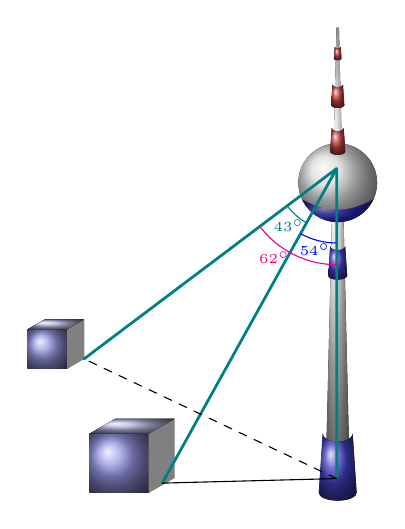
\begin{tikzpicture}[font=\footnotesize,line join=round, line cap=round, >=stealth,scale=0.35] 
			%%%Tháp phát sóng
			\begin{scope}[shift={(-18,-8)},scale=2.25]
				\def\l{5}
				\def\a{0.2}
				\fill[ball color=gray!30](-\a,0)--(-0.1*\a,1.5*\l)--(0.1*\a,1.5*\l)--(\a,0)--cycle;
				\tikzset{vongtron/.pic={
						\fill[ball color=blue!50!gray](-0.95*\a,0.15*\l)arc(180:360:{0.95*\a} and {0.5*\a})--(1.2*\a,0)arc(0:-180:{1.2*\a} and {0.5*\a})--cycle;
				}}
				\tikzset{vongred/.pic={
						\fill[ball color=red!50!gray](-0.95*\a,0.15*\l)arc(180:360:{0.95*\a} and {0.5*\a})--(1.2*\a,0)arc(0:-180:{1.2*\a} and {0.5*\a})--cycle;
				}}
				\tikzset{cau/.pic={
						\def\r{1}
						\fill[ball color=gray!30!white](0,0)circle(\r);
						\fill[ball color=blue,opacity=0.5](-25:\r)arc(-25:-155:\r)[out=-30, in=-150]to(-25:\r);
				}}
				\tikzset{ov/.pic={
						\fill[ball color=gray!40!blue!50!white](0,0)rectangle(1,1);
						\fill[gray](1,1)--++(30:0.5)--++(-90:1)--(1,0)++(30:0.5)coordinate(A);
						\fill[ball color=gray!70!blue!50!white](0,1)--++(30:0.5)--++(1,0)--++(-150:0.5);
				}}
				\path(0,0)pic{vongtron}(0,0.7*\l)pic[scale=0.5]{vongtron}(0,0.96*\l)pic[scale=0.45]{vongtron}(0,\l)pic[scale=0.5]{cau};
				\foreach \i/\m in{1.1/0.4,1.25/0.35,1.4/0.2}
				\path(0,\i*\l)pic[scale=\m]{vongred}(-4,0)pic[scale=0.75]{ov}(-5,2)pic[scale=0.5]{ov};
				\draw[teal,line width=1pt](A)--++(37:5.1)coordinate(B)--++(-119:5.8)coordinate(C)(B)--++(-90:\l)coordinate(D);
				\draw[dashed] (D)--(A);
				\draw(C)--(D);
				\begin{scope}[teal]
					\clip(A)--(B)--(C)--cycle;
					\draw(B)circle(1)++(-130:1.2)node{\tiny $43^\circ$};
				\end{scope}
				\begin{scope}[blue]
					\clip(C)--(B)--(D)--cycle;
					\draw(B)circle(1.2)++(-105:1.35)node{\tiny $54^\circ$};
				\end{scope}
				\begin{scope}[magenta]
					\clip(A)--(B)--(D)--cycle;
					\draw(B)circle(1.55)++(-125:1.75)node{\tiny $62^\circ$};
				\end{scope}
			\end{scope}
	\end{tikzpicture}}	
\shortans{$142$}	
	\loigiai{
		\immini{Gọi các điểm $A$, $B$, $C$, $H$ như hình trên.\\
			Xét tam giác $ABH$ ta có:\\
			$AH=352$, $\widehat{BAH}=62^{\circ}$.\\
			Mà $\cos \widehat{BAH}=\dfrac{AH}{AB} \Rightarrow AB=352 \cdot \cos 62^{\circ} \approx 165{,}25$.\\
			Tương tự, ta có 
			$\cos \widehat{CAH}=\dfrac{AH}{AC} \Rightarrow AC=352 \cdot \cos 54^{\circ} \approx 206{,}9$\\
			Áp dụng định lí côsin cho tam giác $ABC$, ta có
			\allowdisplaybreaks
			\begin{eqnarray*}
				&&BC^2=AB^2+AC^2-2 \cdot AB \cdot AC \cdot \cos A\\ &&\qquad \,=165{,}25^2+206{,}9^2-2\cdot 165{,}25\cdot 206{,}9 \cdot \cos 43^{\circ}\\
				\Rightarrow&& BC \approx 142
			\end{eqnarray*}
			Vậy khoảng cách giữa hai cột mốc này là $142$ m.
		}{
			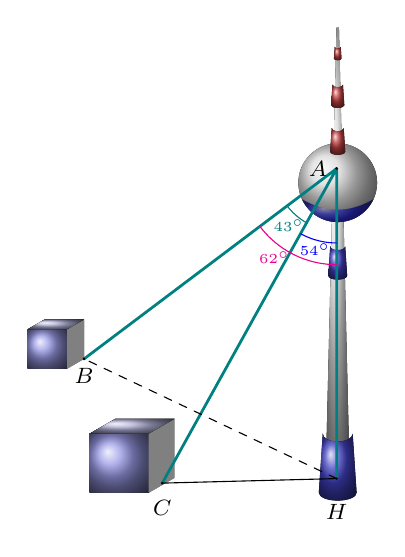
\begin{tikzpicture}[font=\footnotesize,line join=round, line cap=round, >=stealth,scale=0.35] 
				%%%Tháp phát sóng
				\begin{scope}[shift={(-18,-8)},scale=2.25]
					\def\l{5}
					\def\a{0.2}
					\fill[ball color=gray!30](-\a,0)--(-0.1*\a,1.5*\l)--(0.1*\a,1.5*\l)--(\a,0)--cycle;
					\tikzset{vongtron/.pic={
							\fill[ball color=blue!50!gray](-0.95*\a,0.15*\l)arc(180:360:{0.95*\a} and {0.5*\a})--(1.2*\a,0)arc(0:-180:{1.2*\a} and {0.5*\a})--cycle;
					}}
					\tikzset{vongred/.pic={
							\fill[ball color=red!50!gray](-0.95*\a,0.15*\l)arc(180:360:{0.95*\a} and {0.5*\a})--(1.2*\a,0)arc(0:-180:{1.2*\a} and {0.5*\a})--cycle;
					}}
					\tikzset{cau/.pic={
							\def\r{1}
							\fill[ball color=gray!30!white](0,0)circle(\r);
							\fill[ball color=blue,opacity=0.5](-25:\r)arc(-25:-155:\r)[out=-30, in=-150]to(-25:\r);
					}}
					\tikzset{ov/.pic={
							\fill[ball color=gray!40!blue!50!white](0,0)rectangle(1,1);
							\fill[gray](1,1)--++(30:0.5)--++(-90:1)--(1,0)++(30:0.5)coordinate(A);
							\fill[ball color=gray!70!blue!50!white](0,1)--++(30:0.5)--++(1,0)--++(-150:0.5);
					}}
					\path(0,0)pic{vongtron}(0,0.7*\l)pic[scale=0.5]{vongtron}(0,0.96*\l)pic[scale=0.45]{vongtron}(0,\l)pic[scale=0.5]{cau};
					\foreach \i/\m in{1.1/0.4,1.25/0.35,1.4/0.2}
					\path(0,\i*\l)pic[scale=\m]{vongred}(-4,0)pic[scale=0.75]{ov}(-5,2)pic[scale=0.5]{ov};
					\draw[teal,line width=1pt](A)--++(37:5.1)coordinate(B)--++(-119:5.8)coordinate(C)(B)--++(-90:\l)coordinate(D);
					\draw[dashed] (D)--(A);
					\draw(C)--(D);
					\begin{scope}[teal]
						\clip(A)--(B)--(C)--cycle;
						\draw(B)circle(1)++(-130:1.2)node{\tiny $43^\circ$};
					\end{scope}
					\begin{scope}[blue]
						\clip(C)--(B)--(D)--cycle;
						\draw(B)circle(1.2)++(-105:1.35)node{\tiny $54^\circ$};
					\end{scope}
					\begin{scope}[magenta]
						\clip(A)--(B)--(D)--cycle;
						\draw(B)circle(1.55)++(-125:1.75)node{\tiny $62^\circ$};
					\end{scope}
				\end{scope}
				\path  (A) node[below]{$B$};
				\path  (B) node[left]{$A$};
				\path  (C) node[below=0.1cm]{$C$};
				\path  (D) node[below=0.2cm]{$H$};
				\foreach \x/\g in{A/180,B/-90, C/0,D/-90}
				\fill[black](\x) circle (1.5pt);
			\end{tikzpicture}	
	}}
\end{ex}
\begin{ex}%[Nguyễn Tuấn, sáng tác đề HK1 Khối 10]%[0H4C2-2]
	\immini[thm]
	{
		Cho hình vẽ bên, với $M$ là điểm bên trong tam giác sao cho $\widehat{AMB}=\widehat{BMC}=\widehat{CMA}=120^{\circ}$. Đặt $MA=x$, $MB=y$, $MC=z$. Biết các số thực dương $x$, $y$, $z$ thỏa mãn hệ phương trình $\heva{&x^2+y^2+xy=5 \\& y^2+z^2+yz=6\\ &z^2+x^2+zx=7}$. Tính giá trị biểu thức $S=xy+yz+zx$ (kết quả làm tròn đến hàng phần trăm).
		\shortans[]{$5{,}89$}
	}
	{
		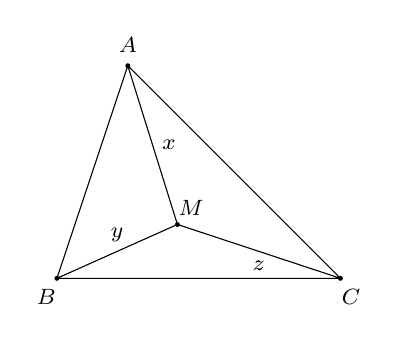
\begin{tikzpicture}[scale=0.9, font=\footnotesize, line join=round, line cap=round,>=stealth]
			\path
			(2,4) coordinate (A)
			(1,1) coordinate (B)
			(5,1) coordinate (C)
			(2.7,1.76) coordinate (M)
			;
			\draw (A)--(B)--(C)--(A)--(M)node[midway,right]{$x$}  (B)--(M)node[midway,above]{$y$} (M)--(C)node[midway,below]{$z$};
			\foreach \x/\g in {A/90,B/-120,C/-60,M/50} 
			\fill[black] (\x) circle (1pt)+(\g:3mm) node {$\x$};
		\end{tikzpicture}
	}
	\loigiai{
		Ta có $AB^2=MA^2+MB^2-2MA\cdot MB\cdot \cos 120^\circ=x^2+y^2+xy=5\Rightarrow AB=\sqrt{5}$.\\
		Tương tự ta tính được $BC=\sqrt{6}$, $CA=\sqrt{7}$.\\
		Đặt $p=\dfrac{AB+BC+AC}{2}=\dfrac{\sqrt{5}+\sqrt{6}+\sqrt{7}}{2}$.\\
		Diện tích tam giác $ABC$ là $S_{ABC}=\sqrt{p\left(p-AB\right)\left(p-AC\right)\left(p-BC\right)}=\sqrt{\dfrac{13}{2}}$.\\
		Ta có $S_{AMB}=\dfrac{1}{2}MA \cdot MB\cdot \sin \widehat{AMB}=\dfrac{\sqrt{3}}{4}xy$, $S_{BMC}=\dfrac{\sqrt{3}}{4}yz$, $S_{CMA}=\dfrac{\sqrt{3}}{4}xz$.\\
		Mà $S_{ABC}=S_{AMB}+S_{BMC}+S_{CMA}=\dfrac{\sqrt{3}}{4}\left(xy+yz+zx\right)$.\\ 
		Thế nên suy ra $xy+yz+zx=\dfrac{2\sqrt{78}}{3}\approx 5{,}89$.
	}
\end{ex}
\Closesolutionfile{ans}
\indapan{6}{ans/ans-CTST_0-OTGK1_De03-KQ}


